\documentclass{article}
\usepackage[margin=1in]{geometry}
\usepackage{amsmath}
\usepackage{amssymb}
\usepackage{amsthm}
\usepackage{bm}
\usepackage{hyperref}
\usepackage{graphicx}
\usepackage{caption}
\usepackage{listings}
\usepackage{xcolor}
\usepackage{float}
\usepackage{placeins}
\graphicspath{{figures/}}

% Code style
\lstdefinestyle{code}{
  basicstyle=\ttfamily\small,
  numbers=left,
  numberstyle=\tiny,
  numbersep=8pt,
  keywordstyle=\color{blue},
  commentstyle=\color{teal!70!black},
  stringstyle=\color{orange!70!black},
  showstringspaces=false,
  breaklines=true,
  frame=single,
  framerule=0.3pt,
  rulecolor=\color{black!15}
}
\lstset{style=code}

\title{Transformer Architecture: Attention, Normalization, Positional Encoding, and Structural Variants}
\author{}
\date{\today}

\begin{document}
\maketitle

\section{Attention Mechanisms}
Self-attention enables transformers to capture pairwise interactions across a sequence without recurrence. Given input matrix $\mathbf{X} \in \mathbb{R}^{T \times d_{\text{model}}}$, linear projections yield queries $\mathbf{Q} = \mathbf{X}\mathbf{W}^Q$, keys $\mathbf{K} = \mathbf{X}\mathbf{W}^K$, and values $\mathbf{V} = \mathbf{X}\mathbf{W}^V$. Scaled dot-product attention computes
\begin{equation}
  \mathrm{Attention}(\mathbf{Q}, \mathbf{K}, \mathbf{V}) = \mathrm{softmax}\left( \frac{\mathbf{Q}\mathbf{K}^{\top}}{\sqrt{d_k}} \right) \mathbf{V},
\end{equation}
where $d_k$ denotes key dimension. The scale $\sqrt{d_k}$ stabilizes gradients. Causal masking applies an additive $-\infty$ mask to enforce autoregressive structure.

\subsection{Multi-Head Attention}
Multi-head attention partitions embeddings into $H$ subspaces, applying attention independently and concatenating:
\begin{align}
  \mathrm{MHA}(\mathbf{X}) &= \mathrm{Concat}( \mathbf{O}_1, \ldots, \mathbf{O}_H ) \mathbf{W}^O, \\
  \mathbf{O}_h &= \mathrm{Attention}\big(\mathbf{X}\mathbf{W}_h^Q, \mathbf{X}\mathbf{W}_h^K, \mathbf{X}\mathbf{W}_h^V\big).
\end{align}
Benefits include richer representation capacity, directional specialization, and the ability to model heterogeneous relations. Key variants include:
\begin{itemize}
  \item \textbf{Relative attention} (Transformer-XL, T5) injecting distance-dependent bias.
  \item \textbf{Sparse attention} (Longformer, BigBird) restricting receptive fields for efficiency.
  \item \textbf{FlashAttention} computing attention in tiles to reduce memory bandwidth.
\end{itemize}
Figure~\ref{fig:self_attention_flow} visualizes the multi-head pipeline, highlighting projection, attention, concatenation, and output mixing.

\subsection{Cross-Attention}
Cross-attention generalizes self-attention by using external context $\mathbf{Y}$ to provide keys and values:
\begin{equation}
  \mathrm{CrossAttn}(\mathbf{X}, \mathbf{Y}) = \mathrm{Attention}(\mathbf{X}\mathbf{W}^Q, \mathbf{Y}\mathbf{W}^K, \mathbf{Y}\mathbf{W}^V).
\end{equation}
Encoder-decoder transformers leverage cross-attention to condition the decoder on encoder outputs, enabling sequence-to-sequence modeling.

\begin{figure}[H]
  \centering
  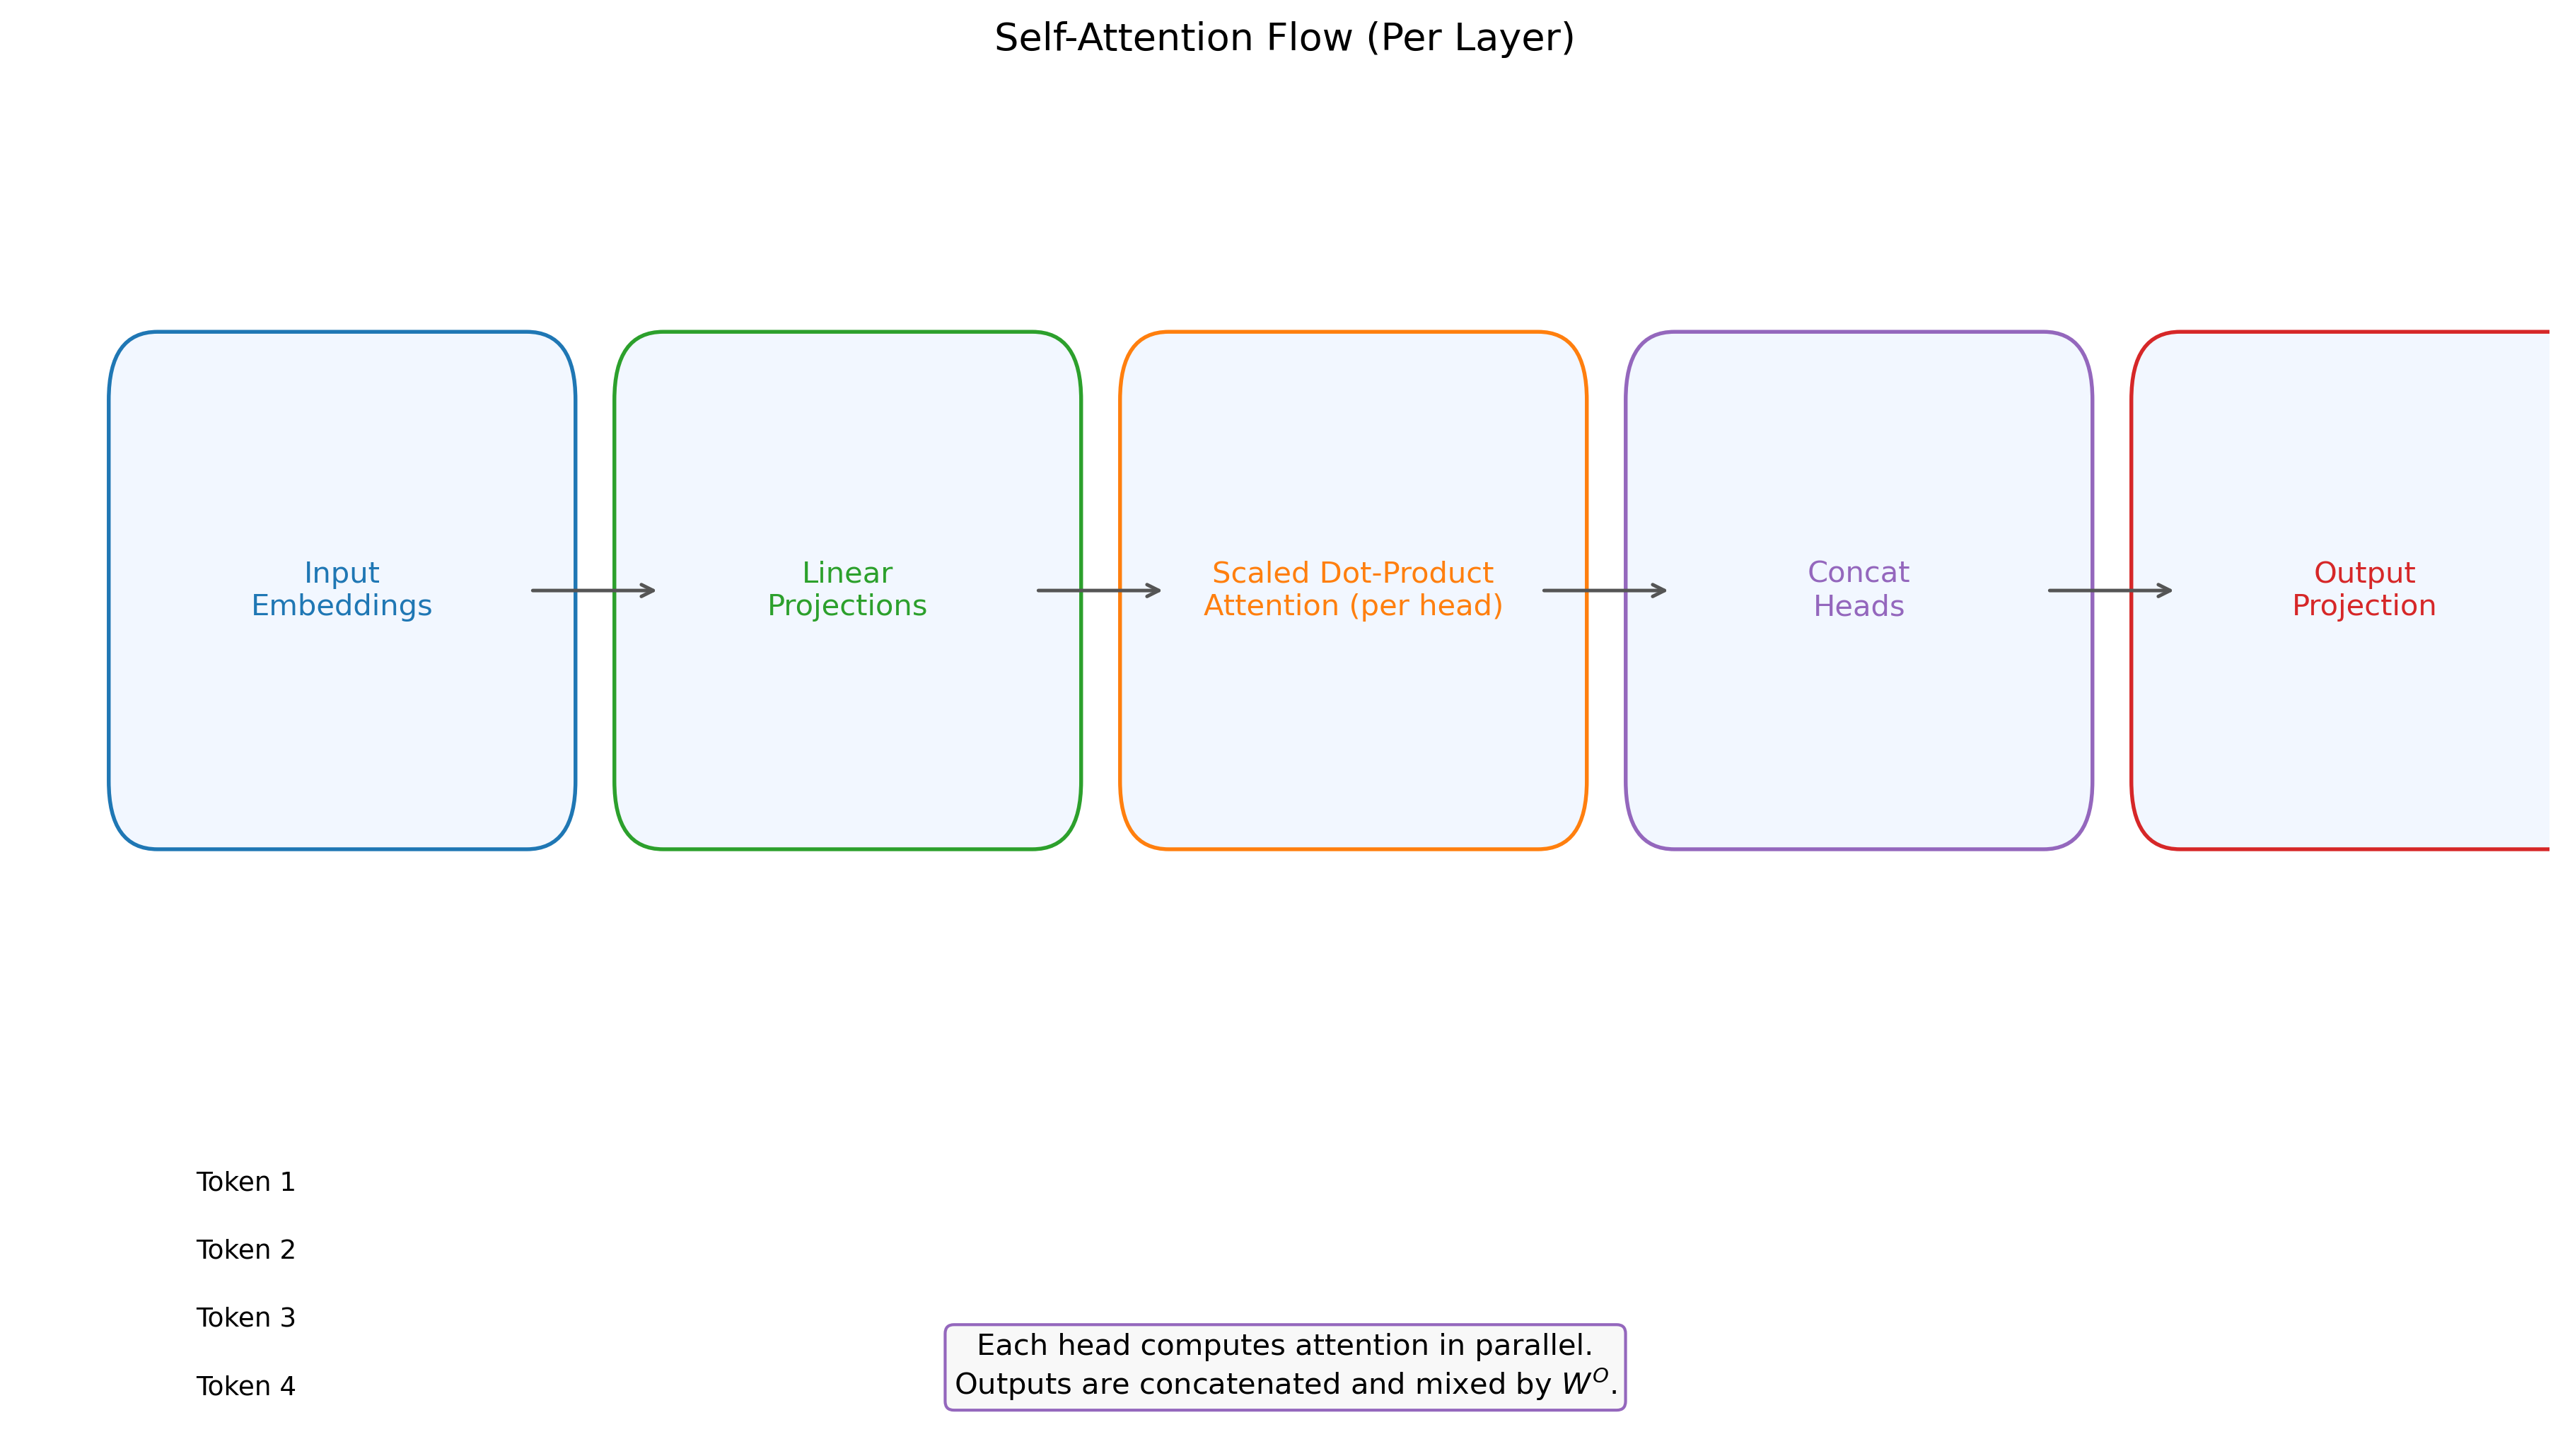
\includegraphics[width=0.85\textwidth]{self_attention_flow.png}
  \caption{Multi-head self-attention pipeline: projection into query/key/value spaces, attention computation per head, concatenation, and output mixing.}
  \label{fig:self_attention_flow}
\end{figure}
\FloatBarrier

\section{Residual Connections and Layer Normalization}
Deep transformers rely on residual pathways and normalization to maintain gradient flow and stable activations.

\subsection{Residual Paths}
Each sublayer (attention or feed-forward network) adds its output to the input:
\begin{equation}
  \mathbf{y} = \mathbf{x} + \mathrm{Sublayer}(\mathbf{x}).
\end{equation}
Residuals mitigate vanishing gradients and allow the network to learn perturbations around identity mappings. Pre-activation placement (Pre-LN) applies normalization before the sublayer, offering training stability for deep stacks.

\subsection{Layer Normalization}
Layer normalization (LayerNorm) standardizes activations per token:
\begin{align}
  \hat{\mathbf{h}} &= \frac{\mathbf{h} - \mu}{\sqrt{\sigma^2 + \epsilon}}, \\
  \mathrm{LayerNorm}(\mathbf{h}) &= \gamma \odot \hat{\mathbf{h}} + \beta,
\end{align}
where $\mu$ and $\sigma^2$ are the mean and variance across features, and $\gamma$, $\beta$ are learnable parameters. Unlike batch normalization, LayerNorm is insensitive to batch size and suits autoregressive decoding. Modern variants (RMSNorm, ScaleNorm) adjust normalization formulae to reduce parameter count or improve stability.

\subsection{Feed-Forward Networks}
Position-wise feed-forward networks (FFN) complement attention:
\begin{equation}
  \mathrm{FFN}(\mathbf{x}) = \sigma(\mathbf{x}\mathbf{W}_1 + \mathbf{b}_1) \mathbf{W}_2 + \mathbf{b}_2.
\end{equation}
Gated linear units (GLU), SwiGLU, and GEGLU introduce multiplicative gating, yielding better throughput-accuracy trade-offs in large models.

\section{Positional Encoding Strategies}
Since attention is permutation-invariant, positional signals inject order information.

\subsection{Sinusoidal Encoding}
Original transformers employed deterministic sinusoids:
\begin{align}
  \mathrm{PE}(t, 2i) &= \sin\left(\frac{t}{10000^{2i/d_{\text{model}}}}\right), \\
  \mathrm{PE}(t, 2i+1) &= \cos\left(\frac{t}{10000^{2i/d_{\text{model}}}}\right).
\end{align}
These encodings generalize to unseen lengths and allow relative distance computation via phase differences.

\subsection{Rotary Position Embeddings (RoPE)}
RoPE rotates query/key vectors by position-dependent angles. For complex embedding $\mathbf{z}_t$, multiplication by a rotation matrix yields
\begin{equation}
  \mathrm{RoPE}(\mathbf{z}_t) = \mathbf{z}_t \cdot e^{i \theta_t}.
\end{equation}
RoPE preserves relative offsets inside inner products, enabling linear extrapolation and efficient extrapolation to longer contexts. Implementations operate on real-valued pairs using rotation matrices.

\subsection{ALiBi Bias}
Attention with Linear Biases (ALiBi) introduces a slope-based bias to the attention logits:
\begin{equation}
  \mathrm{Score}(i, j) = \frac{\mathbf{q}_i^\top \mathbf{k}_j}{\sqrt{d_k}} - m_h (i - j),
\end{equation}
where $m_h$ is a head-specific slope. ALiBi extends context length without additional memory and improves extrapolation by penalizing distant positions in a head-dependent manner.

\section{Encoder and Decoder Structures}
\subsection{Encoder-Decoder (Seq2Seq)}
Encoder-decoder transformers consist of an encoder stack producing latent representations $\mathbf{H}_{\text{enc}}$ and a decoder stack generating outputs conditionally. The decoder contains masked self-attention, cross-attention, and FFN layers. Such architecture excels in translation, summarization, and multi-modal fusion.

\subsection{Decoder-Only Models}
Decoder-only transformers (GPT-class models) drop cross-attention and rely solely on masked self-attention. Their simplicity suits large-scale autoregressive training, and the resulting models act as general-purpose sequence engines via prompting, in-context learning, and alignment fine-tuning.

\subsection{Encoder-Only Models}
Encoder-only architectures (BERT, RoBERTa, DeBERTa) retain bidirectional self-attention without decoding modules. They produce contextual embeddings for understanding tasks and serve as feature extractors or fine-tuned encoders.

\subsection{Mixture and Hybrid Designs}
Modern systems mix components: retrieval-augmented generators add encoder modules to decoder-only backbones; encoder-decoder models sometimes share weights or use prefix tuning for efficient adaptation. Figure~\ref{fig:transformer_stack_variants} compares structural motifs across transformer families.

\begin{figure}[H]
  \centering
  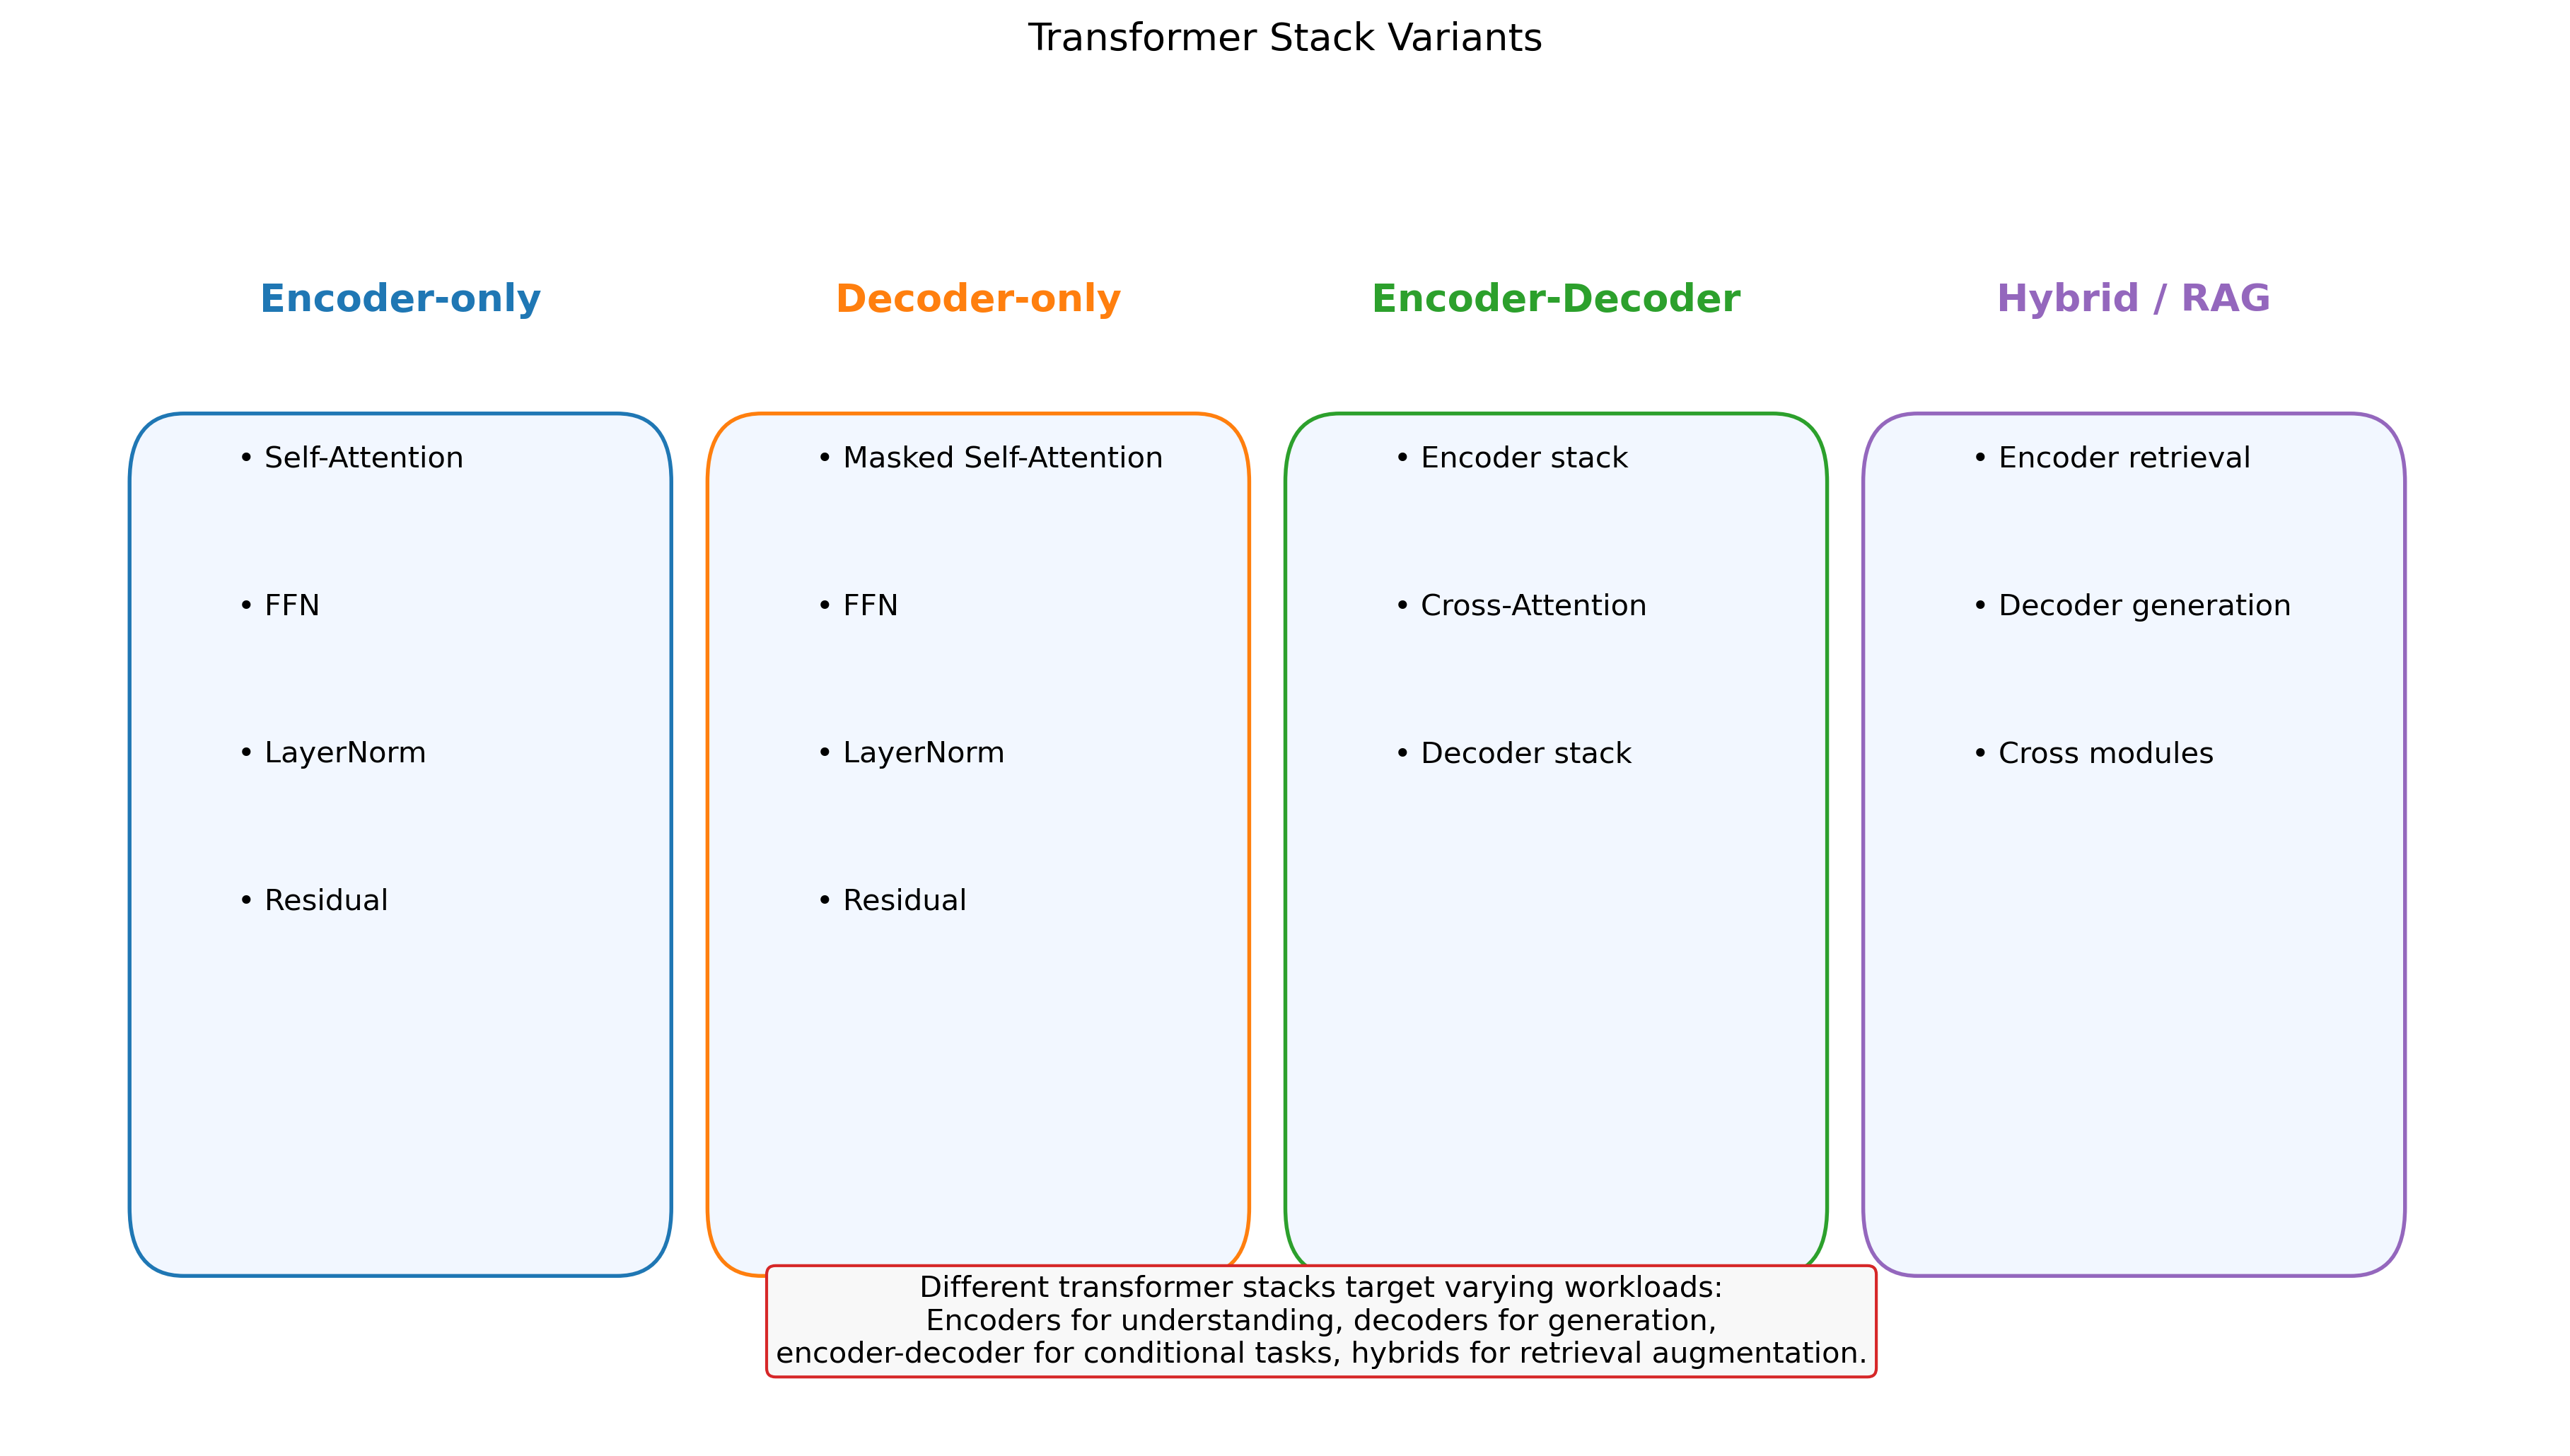
\includegraphics[width=0.9\textwidth]{transformer_stack_variants.png}
  \caption{Structural variants of transformer stacks: encoder-only, decoder-only, encoder-decoder, and hybrid retrieval-augmented designs.}
  \label{fig:transformer_stack_variants}
\end{figure}
\FloatBarrier

\section{Implementation Notes}
\begin{itemize}
  \item \textbf{Scaling laws:} Depth, width, and head count scale with compute budget; post-norm vs. pre-norm choices impact convergence.
  \item \textbf{Regularization:} Dropout, stochastic depth, gradient noise, and weight decay stabilize large models.
  \item \textbf{Hardware:} FlashAttention, tensor parallelism, and quantization reduce memory and latency when deploying transformer blocks.
\end{itemize}

\section*{Further Reading}
\begin{itemize}
  \item Vaswani et al. ``Attention is All You Need.'' NeurIPS 2017.
  \item Shazeer. ``Fast Transformer Decoding: One Write-Head is All You Need.'' 2019.
  \item Xiong et al. ``On Layer Normalization in the Transformer Architecture.'' ICML 2020.
  \item Press et al. ``Train Short, Test Long: Attention with Linear Biases.'' ICLR 2022.
  \item Dao et al. ``FlashAttention: Fast and Memory-Efficient Exact Attention with IO-Awareness.'' NeurIPS 2022.
\end{itemize}

\end{document}
